\begin{savequote}[8cm]
\textlatin{Neque porro quisquam est qui dolorem ipsum quia dolor sit amet, consectetur, adipisci velit...}

There is no one who loves pain itself, who seeks after it and wants to have it, simply because it is pain...
  \qauthor{--- Cicero's \textit{de Finibus Bonorum et Malorum}}
\end{savequote}

\chapter{\label{ch:1-intro}Introduction} 

\minitoc

\section{Motivation}

The body of the project should have, apart from the title, abstract and tables of content:

\begin{itemize}

\item Title page. Your department will have a standard title page form you are required to follow. The title should be informative, contain keywords, and reveal the topic of the thesis. Include the title, author, thesis supervisor, place, and date.

\item Abstract. Briefly state the (1) research problem, (2) methodology, (3) key results, and (4) conclusion. Generally, abstracts are between 100 and 150 words--roughly 5-10 sentences.

\item (What others do?) Chapter 1: Introduction. State (1) the purpose of the investigation, (2) the problem being investigated, (3) the background (context and importance) of the problem (citing previous work by others), (4) your thesis and general approach, and (5) the criteria for your study's success.

\item (What I do?) Chapter 2: Theoretical framework. Develop the theoretical basis for your design or experimental work, including any governing equations. Detailed calculations go to an appendix.

\item (How I do it?) Chapter 3: Methodology. List and describe key materials and apparatus. Then describe the procedure in enough detail that others can duplicate it. For design studies, this section includes component design, fabrication, assembly, and testing procedures. Use illustrations.

\item (What I get?) Chapter 4: Results. Present the results, usually with accompanying tables and graphs. Characterize the patterns and quality of the results and estimate their accuracy and precision. Detailed data go to an appendix. Use analytical graphics.

\item (How I interpret what I get? What I'll to extend this work?) Chapter 5: Discussion, conclusions and future work. Discuss the meaning of the results, stating clearly what their significance is. Compare the results with theoretical expectations and account for anything unexpected.

\end{itemize}

Lorem ipsum dolor sit amet, consectetur adipiscing elit. Maecenas sagittis dolor at nulla feugiat, vitae iaculis est rutrum. Mauris eu sem eros. Sed id faucibus urna. In egestas eros et sapien egestas imperdiet. In hac habitasse platea dictumst.

\begin{mccorrection}
For larger chunks, like this paragraph or indeed entire figures, you can use the \verb|mccorrection| environment.  This environment highlights paragraph-sized and larger blocks with the same blue colour.
\end{mccorrection}

Lorem ipsum dolor sit amet, consectetur adipiscing elit. Maecenas sagittis dolor at nulla feugiat, vitae iaculis est rutrum. Mauris eu sem eros. Sed id faucibus urna. In egestas eros et sapien egestas imperdiet. In hac habitasse platea dictumst.

\section{Equations}

Lorem ipsum dolor sit amet, consectetur adipiscing elit. Maecenas sagittis dolor at nulla feugiat, vitae iaculis est rutrum. Mauris eu sem eros. Sed id faucibus urna. In egestas eros et sapien egestas imperdiet. In hac habitasse platea dictumst. Phasellus vitae varius tortor. Mauris nec sollicitudin enim. Suspendisse molestie leo nec mauris molestie, nec imperdiet magna vehicula. Phasellus sodales tortor dui, a lacinia turpis congue at. Pellentesque mattis dui non libero commodo, at accumsan ex ultrices. Integer eget ex eget dui cursus euismod et accumsan felis. Nullam laoreet sodales dui, ut finibus elit varius a. Sed elementum orci quis libero ullamcorper, eget egestas enim convallis. Sed nibh libero, tincidunt ultricies nibh quis, lobortis placerat mauris. Maecenas at laoreet risus, nec dictum libero. Donec accumsan, orci eu tempus mattis, nisl arcu auctor turpis, ac sollicitudin justo orci nec nulla.

\begin{equation}
\boldsymbol{n}^{\otimes d}_1=\tfrac{1}{2}\begin{bmatrix}\tfrac{1}{3}-\cos2\psi & \sin2\psi & 0 \\
\sin2\psi & \tfrac{1}{3}+\cos2\psi & 0 \\
0 & 0 & -\tfrac{2}{3} \\
\end{bmatrix}
\end{equation}


\section{Algorithms}

 \begin{algorithm}
 \caption{Calculate $y = x^n$}
 \label{alg1}
 \begin{algorithmic}
 \REQUIRE $n \geq 0 \vee x \neq 0$
 \ENSURE $y = x^n$
 \STATE $y \leftarrow 1$
 \IF{$n < 0$}
 \STATE $X \leftarrow 1 / x$
 \STATE $N \leftarrow -n$
 \ELSE
 \STATE $X \leftarrow x$
 \STATE $N \leftarrow n$
 \ENDIF
 \WHILE{$N \neq 0$}
 \IF{$N$ is even}
 \STATE $X \leftarrow X \times X$
 \STATE $N \leftarrow N / 2$
 \ELSE[$N$ is odd]
 \STATE $y \leftarrow y \times X$
 \STATE $N \leftarrow N - 1$
 \ENDIF
 \ENDWHILE
 \end{algorithmic}
 \end{algorithm}
 
Lorem ipsum dolor sit amet, consectetur adipiscing elit. Maecenas sagittis dolor at nulla feugiat, vitae iaculis est rutrum. Mauris eu sem eros. Sed id faucibus urna. In egestas eros et sapien egestas imperdiet. In hac habitasse platea dictumst. Phasellus vitae varius tortor. Mauris nec sollicitudin enim. Suspendisse molestie leo nec mauris molestie, nec imperdiet magna vehicula. Phasellus sodales tortor dui, a lacinia turpis congue at. Pellentesque mattis dui non libero commodo, at accumsan ex ultrices. Integer eget ex eget dui cursus euismod et accumsan felis. Nullam laoreet sodales dui, ut finibus elit varius a. Sed elementum orci quis libero ullamcorper, eget egestas enim convallis. Sed nibh libero, tincidunt ultricies nibh quis, lobortis placerat mauris. Maecenas at laoreet risus, nec dictum libero. Donec accumsan, orci eu tempus mattis, nisl arcu auctor turpis, ac sollicitudin justo orci nec nulla.

\clearpage

\section{Python code}

\begin{lstlisting}[language=Python, caption=Python example]
import numpy as np
    
def incmatrix(genl1,genl2):
    m = len(genl1)
    n = len(genl2)
    M = None #to become the incidence matrix
    VT = np.zeros((n*m,1), int)  #dummy variable
    
    #compute the bitwise xor matrix
    M1 = bitxormatrix(genl1)
    M2 = np.triu(bitxormatrix(genl2),1) 

    for i in range(m-1):
        for j in range(i+1, m):
            [r,c] = np.where(M2 == M1[i,j])
            for k in range(len(r)):
                VT[(i)*n + r[k]] = 1;
                VT[(i)*n + c[k]] = 1;
                VT[(j)*n + r[k]] = 1;
                VT[(j)*n + c[k]] = 1;
                
                if M is None:
                    M = np.copy(VT)
                else:
                    M = np.concatenate((M, VT), 1)
                
                VT = np.zeros((n*m,1), int)
    
    return M
\end{lstlisting}

Nam eget sem sed ligula vehicula iaculis. In non arcu a nisl interdum gravida. Nam egestas erat non turpis sagittis vestibulum. Praesent est metus, facilisis eu commodo sed, sagittis et est. Duis scelerisque luctus erat, elementum pulvinar felis bibendum a. Morbi hendrerit rhoncus consectetur. Vestibulum nec odio finibus, blandit turpis eget, dignissim orci. Curabitur eu ligula auctor, porttitor nulla non, maximus turpis. Nunc sed quam at est varius interdum eu vitae odio. Vestibulum egestas dapibus nulla sit amet fermentum.

Vestibulum ut neque urna. Ut nec odio lobortis, ultricies nulla quis, ultricies tellus. Nam ac iaculis sapien. Vivamus vitae risus id tortor interdum pellentesque. Quisque lorem lectus, sagittis vel metus et, sagittis finibus justo. Curabitur pulvinar odio tellus, eu vehicula est dictum eget. Morbi sed justo justo. Vivamus enim nibh, facilisis pretium luctus quis, ullamcorper quis ipsum. Pellentesque a mi a elit euismod malesuada.

\section{Julia code}

\begin{lstlisting}[language=Julia, caption=Julia example]
#= This is a code sample for the Julia language
(adapted from http://julialang.org) =#
function mandel(z)
    c = z
    maxiter = 80
    for n = 1:maxiter
        if abs(z) > 2
            return n-1
        end
        z = z^2 + c
    end
    return maxiter
end

function helloworld()
    println("Hello, World!") # Bye bye, MATLAB!
end

function randmatstat(t)
    n = 5
    v = zeros(t)
    w = zeros(t)
    for i = 1:t
        a = randn(n,n)
        b = randn(n,n)
        c = randn(n,n)
        d = randn(n,n)
        P = [a b c d]
        Q = [a b; c d]
        v[i] = trace((P.'*P)^4)
        w[i] = trace((Q.'*Q)^4)
    end
    std(v)/mean(v), std(w)/mean(w)
end
\end{lstlisting}


Vestibulum interdum est vel orci tincidunt auctor. Nunc tristique nulla nec blandit fermentum. Maecenas id libero ut justo dictum sodales. Nullam justo sapien, dignissim vel enim at, porta pharetra metus. Integer euismod quam eget ligula gravida euismod. Pellentesque commodo, quam sit amet bibendum tempor, nisi odio varius mauris, et accumsan justo ex sed nunc. Cras bibendum nibh ac dolor volutpat, non elementum orci pulvinar. Maecenas et porttitor nulla. Suspendisse sapien massa, dapibus at blandit et, rhoncus suscipit velit. Fusce molestie, velit eget sagittis suscipit, est libero aliquam libero, in iaculis mi tellus ac nunc.

\section{Matlab code}

\begin{lstlisting}[language=Matlab, caption=Matlab example]
for i = 1:3
    if i >= 5                   % literate programming replacement
        disp('cool');          % comment with some mcommentfont
    end
    [~,ind] = max(vec);
    x_last = x(1,end);
    v(end);
    really really long really really long really really long really really long really really long line % blaaaaaaaa
end
\end{lstlisting}

Sed in rhoncus lectus. Mauris vulputate purus non malesuada pulvinar. Curabitur ullamcorper hendrerit elit, id vulputate libero sagittis vel. Pellentesque ac faucibus est. Class aptent taciti sociosqu ad litora torquent per conubia nostra, per inceptos himenaeos. Integer venenatis, nisl eleifend pellentesque consequat, sem tortor malesuada ante, ut tincidunt elit tortor sit amet nunc.

Cras vehicula ipsum sit amet dui rutrum ultrices. Integer eu eleifend odio. Praesent tempor, libero id ullamcorper euismod, lectus diam lobortis mauris, id venenatis arcu sem vitae purus. Pellentesque luctus tristique metus quis mollis. Praesent ullamcorper neque velit, sed iaculis est convallis sit amet. Quisque nec massa ut magna lobortis imperdiet. Quisque rhoncus purus eget mollis aliquet. Donec vehicula viverra nisl, sed posuere turpis vulputate non. Donec malesuada, eros id interdum volutpat, ipsum orci luctus quam, non pulvinar urna ipsum eget purus. Nam hendrerit condimentum tristique.
Proin metus velit, tempor at fringilla non, dictum eu felis. 

\section{OpenScad code (3D design)}

\begin{lstlisting}[language=OpenSCAD, caption=OpenSCAD example.]
$fn=6;
marg=0.98;
//draw segment between 2 specified points
module rod(p1,p2,r){ 
    translate((p1+p2)/2)
        rotate([-acos((p2[2]-p1[2]) / norm(p1-p2)),0,
        -atan2(p2[0]-p1[0],p2[1]-p1[1])])
            cylinder(r1=r, r2=r, h=norm(p1-p2), center=true);
}
//geometry definition
translate([-41,-101,28])
    sphere(r=0.202);
rod([-41,-101,28],[-41,-101,31],marg*0.202);
rod([-41,-101,28],[-41,-98,28],marg*0.202);
rod([-41,-101,28],[-38,-101,28],marg*0.202);

\end{lstlisting}

Morbi eu lectus arcu. Sed fringilla dui ut magna commodo, a malesuada ante pellentesque. Donec ornare facilisis pellentesque. Nulla vitae fringilla velit. Nunc id tellus nisl. Maecenas pretium elit lectus, nec consectetur nunc vulputate et. Sed facilisis magna nec gravida hendrerit. Sed a cursus nisl, in rhoncus massa. Curabitur ut nibh interdum, tempor risus vel, scelerisque nibh. Mauris quis ipsum sed risus tempor convallis ut a eros.

\section{BDF code. Used in Nastran}

\begin{lstlisting}[language=BDF, caption=BDF example.]
ID,WIRES,SIZ40
SOL,101
TIME,5
CEND
TITLE=GENERATIVE METAMATERIAL
SUBTITLE=CASE 1
LOAD=10
SPC=11
DISP=ALL
STRESS=ALL
STRAIN=ALL
ELFORCE=ALL
SPCFORCE=ALL
PARAM,BAILOUT,-1
BEGIN BULK
MDLPRM,HDF5,0

$ NODES COME HERE

GRID,1,,0.0,0.0,0.0
GRID,2,,0.0,10.0,0.0
GRID,3,,10.0,10.0,0.0
GRID,4,,10.0,0.0,0.0

$ ELEMENTS COME HERE

CBAR,1,11,1,2,1.0,0.0,0.0
CBAR,2,12,2,3,1.0,1.0,0.0
CBAR,3,13,3,4,1.0,0.0,0.0
CBAR,4,12,4,1,1.0,1.0,0.0

$ GEO/MECH PROPS COME HERE

PBARL,11,21,,BAR
,0.75,0.75,,
PBARL,12,21,,BAR
,0.8,0.8,,
PBARL,13,21,,BAR
,0.84,0.84,,

MAT1,21,21e4,,0.3

$ BC AND LOADS COME HERE

FORCE,10,3,,15.0,0.0,0.0,-1.0

SPC1,11,123456,1
SPC1,11,123456,2
\end{lstlisting}

Morbi eu lectus arcu. Sed fringilla dui ut magna commodo, a malesuada ante pellentesque. Donec ornare facilisis pellentesque. Nulla vitae fringilla velit. Nunc id tellus nisl. Maecenas pretium elit lectus, nec consectetur nunc vulputate et. Sed facilisis magna nec gravida hendrerit. Sed a cursus nisl, in rhoncus massa. Curabitur ut nibh interdum, tempor risus vel, scelerisque nibh. Mauris quis ipsum sed risus tempor convallis ut a eros.

\section{VTU code. Used in Paraview}

\begin{lstlisting}[language=VTU, caption=VTU example.]
<?xml version="1.0"?> 
	<VTKFile type="UnstructuredGrid">
		<UnstructuredGrid>
			<Piece NumberOfPoints="4"  NumberOfCells="4"> 
				<Points>
					<DataArray type="Float64" NumberOfComponents="3" format="ascii">
0.0     0.0     0.0
0.0     10.0    0.0
10.0    10.0    0.0
10.0    0.0     0.0
					</DataArray>
				</Points>
				<Cells>
				    <DataArray type="Int32" Name="connectivity" format="ascii">
1 2
2 3
3 4
4 1
					</DataArray>
					<DataArray type="Int32" Name="offsets" format="ascii">
2
4
6
8
					</DataArray>
					<DataArray type="UInt8" Name="types" format="ascii">
3
3
3
3
					</DataArray>
				</Cells>
				<CellData>
					<DataArray type="Float64" Name="Radius" NumberOfComponents="1" format="ascii">
0.1
0.2
0.3
0.4
					</DataArray>
					<DataArray type="Float64" Name="Young Modulus" NumberOfComponents="1" format="ascii">
100
115
150
200
					</DataArray>
				</CellData>
			</Piece>
		</UnstructuredGrid>
	</VTKFile>

\end{lstlisting}

Morbi eu lectus arcu. Sed fringilla dui ut magna commodo, a malesuada ante pellentesque. Donec ornare facilisis pellentesque. Nulla vitae fringilla velit. Nunc id tellus nisl. Maecenas pretium elit lectus, nec consectetur nunc vulputate et. Sed facilisis magna nec gravida hendrerit. Sed a cursus nisl, in rhoncus massa. Curabitur ut nibh interdum, tempor risus vel, scelerisque nibh. Mauris quis ipsum sed risus tempor convallis ut a eros.

\section{STL code. Used for 3D printing}

Morbi eu lectus arcu. Sed fringilla dui ut magna commodo, a malesuada ante pellentesque. Donec ornare facilisis pellentesque. Nulla vitae fringilla velit. Nunc id tellus nisl. Maecenas pretium elit lectus, nec consectetur nunc vulputate et. Sed facilisis magna nec gravida hendrerit. Sed a cursus nisl, in rhoncus massa. Curabitur ut nibh interdum, tempor risus vel, scelerisque nibh. Mauris quis ipsum sed risus tempor convallis ut a eros.

\begin{lstlisting}[language=STL, caption=STL example.]
solid "OpenSCAD"
 facet normal -0.944150984287 -0.329513221979 0
  outer loop
   vertex -44.2175102234 -28.7303390503 17.0843906403
   vertex -40 -25 4.99999952316
   vertex -40 -30 4.99999952316
  endloop
 endfacet
endsolid "OpenSCAD"

\end{lstlisting}

Morbi eu lectus arcu. Sed fringilla dui ut magna commodo, a malesuada ante pellentesque. Donec ornare facilisis pellentesque. Nulla vitae fringilla velit. Nunc id tellus nisl. Maecenas pretium elit lectus, nec consectetur nunc vulputate et. Sed facilisis magna nec gravida hendrerit. Sed a cursus nisl, in rhoncus massa. Curabitur ut nibh interdum, tempor risus vel, scelerisque nibh. Mauris quis ipsum sed risus tempor convallis ut a eros.

\section{DOS code}

Morbi eu lectus arcu. Sed fringilla dui ut magna commodo, a malesuada ante pellentesque. Donec ornare facilisis pellentesque. Nulla vitae fringilla velit. Nunc id tellus nisl. Maecenas pretium elit lectus, nec consectetur nunc vulputate et. Sed facilisis magna nec gravida hendrerit. Sed a cursus nisl, in rhoncus massa. Curabitur ut nibh interdum, tempor risus vel, scelerisque nibh. Mauris quis ipsum sed risus tempor convallis ut a eros.


\begin{mdframed}[backgroundcolor=black,leftmargin=0.5cm,hidealllines=true,%
  innerleftmargin=0.2cm,innerrightmargin=0.2cm,innertopmargin=-0.1cm,innerbottommargin=-0.85cm]

\begin{lstlisting}[language=DOS, caption={MSE runtime example}]
  METAMATERIAL STL SLICER ENGINE
------------- v 0.1 -------------

--------- DEFINE PARAMS ---------
Define grid size, higher means smaller cells (int):
25

Define n of PBARL sizes, higher means smoother cells (int):
Default (15)

Output file format (BDF or SCAD or VTU or ALL):
Default (ALL)

Cell type (c or d or any combination):
cd

Define Young Modulus (int):
210000

Define boundary conditions case (0=None):
2

----------- EXECUTION -----------
Grid is: 24x24x27
Creating node cloud...
Getting mechanical properties in each node...
Generating "MSE_24x24x27_15-c.bdf" file...
Generating "MSE_24x24x27_15-d.bdf" file...
Generating "MSE_24x24x27_15-c.scad" file...
Generating "MSE_24x24x27_15-d.scad" file...
Generating "MSE_24x24x27_15-c.vtu" file...
Generating "MSE_24x24x27_15-d.vtu" file...

\end{lstlisting}
\end{mdframed}


Morbi eu lectus arcu. Sed fringilla dui ut magna commodo, a malesuada ante pellentesque. Donec ornare facilisis pellentesque. Nulla vitae fringilla velit. Nunc id tellus nisl. Maecenas pretium elit lectus, nec consectetur nunc vulputate et. Sed facilisis magna nec gravida hendrerit. Sed a cursus nisl, in rhoncus massa. Curabitur ut nibh interdum, tempor risus vel, scelerisque nibh. Mauris quis ipsum sed risus tempor convallis ut a eros.

\section{Tables}

Cras vehicula ipsum sit amet dui rutrum ultrices. Integer eu eleifend odio. Praesent tempor, libero id ullamcorper euismod, lectus diam lobortis mauris, id venenatis arcu sem vitae purus. Pellentesque luctus tristique metus quis mollis. Praesent ullamcorper neque velit, sed iaculis est convallis sit amet. Quisque nec massa ut magna lobortis imperdiet. Quisque rhoncus purus eget mollis aliquet. Donec vehicula viverra nisl, sed posuere turpis vulputate non. Donec malesuada, eros id interdum volutpat, ipsum orci luctus quam, non pulvinar urna ipsum eget purus. Nam hendrerit condimentum tristique.

\begin{table}[ht]
  \centering
  \caption{Tabla sobre XXXX.}
  \label{tab:Dam}
  \footnotesize\sffamily
  \begin{tabular}{|l|c|c|c|c|c|c|}
\hline
    \textbf{AAA} & Total & \cellcolor{codegreen!50}Cent. & \cellcolor{codegreen!50}Rod. izda & \cellcolor{gray!50}Cent.  & \cellcolor{gray!50}Rod. dcha & \cellcolor{gray!50}Arcn \\
    \hline
   \cellcolor{gray!50} Long (m) & 12.98 & 2.93 & 7.33 & 2.16 & 3.48 &  3.34 \\
    \hline
    \cellcolor{gray!50} Long (m) & 5.76 & 1.02 & 2.39 & 1.78 & 1.12 &  0.74\\
    \hline
    \cellcolor{gray!50} Tama (cm) & 40.07 & 0.0 & 0.0 & 40.28 & 40.28 &  39.65 \\
    \hline
    \cellcolor{gray!50} Super (\%) & 26.54 & 0.0 & 0.0 & 44.32 & 44.32 &  44.03 \\
    \hline
   \cellcolor{gray!50} Estado global & \cellcolor{codegreen!60}  &  \cellcolor{blue!60}& \cellcolor{codegreen!60}&\cellcolor{yellow!60} &\cellcolor{codegreen!60}& \cellcolor{codegreen!60} \\
        \hline
  \end{tabular}
\end{table}

Proin volutpat enim ut fermentum aliquam. Nam dictum nisi eu nisl viverra fermentum. Pellentesque tristique arcu non orci congue faucibus. Fusce sit amet nisl fringilla, feugiat turpis vitae, eleifend ante. Suspendisse elementum, lectus non pulvinar bibendum, lectus massa faucibus turpis, vitae porta risus sem quis metus. Maecenas id sapien et dui lobortis imperdiet nec eu mi. Quisque porttitor tincidunt nisi, eget sagittis orci. Nunc mattis erat malesuada facilisis viverra. Maecenas sodales iaculis nisi vel tincidunt. Morbi aliquet nibh ac facilisis consectetur. In ultrices libero quis massa porttitor cursus. Quisque suscipit ac tortor eget aliquet. Ut eget lacus vel orci viverra maximus at at purus.

\begin{table}[ht]
  \centering
  \caption{Tabla 2 sobre XXXX.}
  \label{tab:Dam2}
  \footnotesize\sffamily
\begin{tabular}{ |c|c|c|  }
\hline
\rowcolor{lightgray} \multicolumn{3}{|c|}{Country List} \\
\hline
Country Name     or Area Name& ISO ALPHA 2 Code &ISO ALPHA 3 \\
\hline
Afghanistan & AF &AFG \\
\rowcolor{gray}
Aland Islands & AX  & ALA \\
Albania    &AL & ALB \\
Algeria   &DZ & DZA \\
American Samoa & AS & ASM \\
Andorra & AD & \cellcolor[HTML]{AA0044} AND \\
Angola & AO & AGO \\
\hline
\end{tabular}
\end{table}

Cras vehicula ipsum sit amet dui rutrum ultrices. Integer eu eleifend odio. Praesent tempor, libero id ullamcorper euismod, lectus diam lobortis mauris, id venenatis arcu sem vitae purus. Pellentesque luctus tristique metus quis mollis. Praesent ullamcorper neque velit, sed iaculis est convallis sit amet. Quisque nec massa ut magna lobortis imperdiet. Quisque rhoncus purus eget mollis aliquet. Donec vehicula viverra nisl, sed posuere turpis vulputate non. Donec malesuada, eros id interdum volutpat, ipsum orci luctus quam, non pulvinar urna ipsum eget purus. Nam hendrerit condimentum tristique.

\section{Graphs and figures}

Nam massa neque, varius nec suscipit id, cursus ac mi. Cum sociis natoque penatibus et magnis dis parturient montes, nascetur ridiculus mus. 

\begin{figure}[H]
\centering
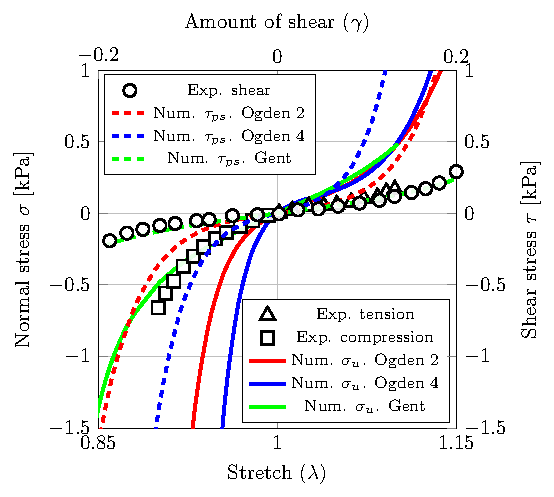
\includegraphics[width=0.7\textwidth]{figures/chapter_1/graphs/Corona_radiata/graph_corona_radiata.pdf}
\caption[tab]{Experimental and analytical comparison.}
\label{fig:corona_radiata}
\end{figure}

In hac habitasse platea dictumst. Vivamus facilisis nunc quis dictum consectetur. Sed congue sed magna non auctor. Vestibulum accumsan sit amet erat non congue. Sed at condimentum mi, sed scelerisque urna. Etiam tristique pulvinar rutrum. Donec semper nulla vitae rutrum semper. Maecenas ultrices nibh at orci sodales tincidunt sit amet vitae arcu. Curabitur interdum tincidunt ipsum, nec tincidunt nunc dapibus in. Nunc sit amet elementum massa, ut ornare lacus. Vivamus convallis fringilla erat, non suscipit sapien convallis eu. Nunc viverra lectus sit amet turpis viverra, eget iaculis purus rhoncus.

Nam massa neque, varius nec suscipit id, cursus ac mi. Cum sociis natoque penatibus et magnis dis parturient montes, nascetur ridiculus mus. In hac habitasse platea dictumst. Vivamus facilisis nunc quis dictum consectetur. Sed congue sed magna non auctor. Vestibulum accumsan sit amet erat non congue. Sed at condimentum mi, sed scelerisque urna. Etiam tristique pulvinar rutrum. Donec semper nulla vitae rutrum semper. Maecenas ultrices nibh at orci sodales tincidunt sit amet vitae arcu. Curabitur interdum tincidunt ipsum, nec tincidunt nunc dapibus in. Nunc sit amet elementum massa, ut ornare lacus. Vivamus convallis fringilla erat, non suscipit sapien convallis eu. Nunc viverra lectus sit amet turpis viverra, eget iaculis purus rhoncus.

\begin{figure}[H]
\centering
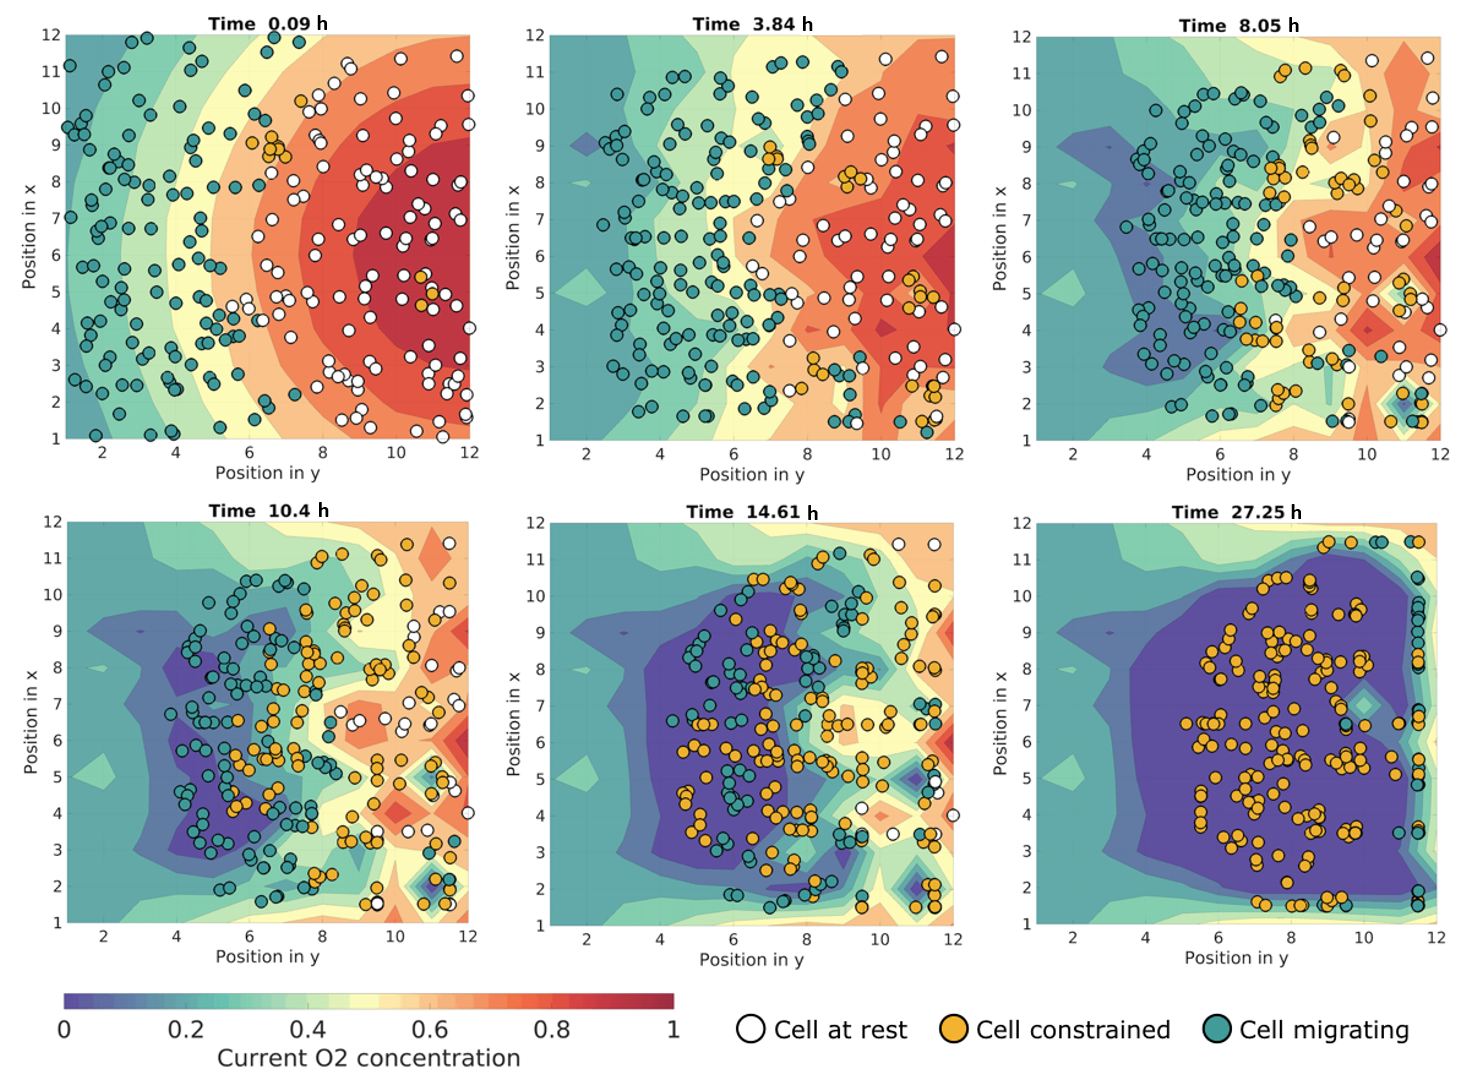
\includegraphics[width=1.0\textwidth]{figures/chapter_1/images/lateral}
\caption[tab]{Results.}
\label{fig:results}
\end{figure}

In hac habitasse platea dictumst. Vivamus facilisis nunc quis dictum consectetur. Sed congue sed magna non auctor. Vestibulum accumsan sit amet erat non congue. Sed at condimentum mi, sed scelerisque urna. Etiam tristique pulvinar rutrum. Donec semper nulla vitae rutrum semper. Maecenas ultrices nibh at orci sodales tincidunt sit amet vitae arcu. Curabitur interdum tincidunt ipsum, nec tincidunt nunc dapibus in. Nunc sit amet elementum massa, ut ornare lacus. Vivamus convallis fringilla erat, non suscipit sapien convallis eu. Nunc viverra lectus sit amet turpis viverra, eget iaculis purus rhoncus.

Nam massa neque, varius nec suscipit id, cursus ac mi. Cum sociis natoque penatibus et magnis dis parturient montes, nascetur ridiculus mus. In hac habitasse platea dictumst. Vivamus facilisis nunc quis dictum consectetur. Sed congue sed magna non auctor. Vestibulum accumsan sit amet erat non congue. Sed at condimentum mi, sed scelerisque urna. Etiam tristique pulvinar rutrum. Donec semper nulla vitae rutrum semper. Maecenas ultrices nibh at orci sodales tincidunt sit amet vitae arcu. Curabitur interdum tincidunt ipsum, nec tincidunt nunc dapibus in. Nunc sit amet elementum massa, ut ornare lacus. Vivamus convallis fringilla erat, non suscipit sapien convallis eu. Nunc viverra lectus sit amet turpis viverra, eget iaculis purus rhoncus.

\section{Citations}

In hac habitasse platea dictumst. Vivamus facilisis nunc quis dictum consectetur. Sed congue sed magna non auctor. Vestibulum accumsan sit amet erat non congue. Sed at condimentum mi, sed scelerisque urna. Etiam tristique pulvinar rutrum. Donec semper nulla vitae rutrum semper. Maecenas ultrices nibh at orci sodales tincidunt sit amet vitae arcu. Curabitur interdum tincidunt ipsum, nec tincidunt nunc dapibus in. Nunc sit amet elementum massa, ut ornare lacus. Vivamus convallis fringilla erat, non suscipit sapien convallis eu. Nunc viverra lectus sit amet turpis viverra, eget iaculis purus rhoncus.

Cite.. \cite{Murphy16,50Shades}

Nam massa neque, varius nec suscipit id, cursus ac mi. Cum sociis natoque penatibus et magnis dis parturient montes, nascetur ridiculus mus. In hac habitasse platea dictumst. Vivamus facilisis nunc quis dictum consectetur. Sed congue sed magna non auctor. Vestibulum accumsan sit amet erat non congue. Sed at condimentum mi, sed scelerisque urna. Etiam tristique pulvinar rutrum. Donec semper nulla vitae rutrum semper. Maecenas ultrices nibh at orci sodales tincidunt sit amet vitae arcu. Curabitur interdum tincidunt ipsum, nec tincidunt nunc dapibus in. Nunc sit amet elementum massa, ut ornare lacus. Vivamus convallis fringilla erat, non suscipit sapien convallis eu. Nunc viverra lectus sit amet turpis viverra, eget iaculis purus rhoncus.